% This is samplepaper.tex, a sample chapter demonstrating the
% LLNCS macro package for Springer Computer Science proceedings;
% Version 2.20 of 2017/10/04
%
\documentclass[runningheads]{llncs}
%
\usepackage{caption}
\usepackage{subcaption}
\usepackage{todonotes}
\usepackage{amsmath}
\usepackage{url}
\usepackage{graphicx}
\usepackage{hyperref}
% Used for displaying a sample figure. If possible, figure files should
% be included in EPS format.
%
% If you use the hyperref package, please uncomment the following line
% to display URLs in blue roman font according to Springer's eBook style:
% \renewcommand\UrlFont{\color{blue}\rmfamily}

\begin{document}
%
\title{Medical Image Analysis Assignment 2}
%
%\titlerunning{Abbreviated paper title}
% If the paper title is too long for the running head, you can set
% an abbreviated paper title here
%
\author{Casper Bresdahl}
%
% \authorrunning{F. Author et al.}
% First names are abbreviated in the running head.
% If there are more than two authors, 'et al.' is used.
%
% \institute{Princeton University, Princeton NJ 08544, USA \and
% Springer Heidelberg, Tiergartenstr. 17, 69121 Heidelberg, Germany
% \email{lncs@springer.com}\\
% \url{http://www.springer.com/gp/computer-science/lncs} \and
% ABC Institute, Rupert-Karls-University Heidelberg, Heidelberg, Germany\\
% \email{\{abc,lncs\}@uni-heidelberg.de}}
%
\maketitle              % typeset the header of the contribution
%
\section{Introduction}
This week we will first introduce the theory behind advection and mean curvature flow and how we can discretize these. We will then look at the first experiment looking into how advection without any boundary issues behave compared to advection where boundaries will play a role. We will then look at the second experiment where we will compare three different boundary conditions and how these change the end result when applying mean curvature flow to a signed distance field. At the end we will conclude on our results.
\section{Medical image segmentation}
Segmentation is widely used in medical image analysis where knowledge of an object's shape, size or volume is needed. It could be there is a suspicion that a patient's heart is enlarged, then finding the shape of the heart from an x-ray image would allow for easy measurement of its size. However, this would require someone to draw the shape of the heart from that x-ray scan. With the development of segmentation algorithms this can now be automated. Medical image segmentation can also be used for imaged guided procedures, where a surgeon would have to operate with great precision, for example when inserting pronator screws. Medical image segmentation is also, as touched upon before, more broadly used for computer aided diagnosis where perhaps the shape of a patient's organs is measured and used for a diagnosis. Other examples would be to apply thresholding on a CT image to extract the bones, to apply Region growing in mammograms in order to extract a potential lesion from its background, and to separate different tissues from each other based on EM results \cite{otherExamples}.

%But how is medical image segmentation achieved? There are numerous methods all with their own pros and cons. Some of them will be discussed in the following.\\
%\textbf{Histogram thresholding} is a strong tool to identify objects based on their relative intensity to other objects in an image. In an image with high contrast, the background might be black while the object we would like to segment is completely white, then the histogram of this image would show two strong peaks in the lower and upper intensities. Knowing the object we want to segment is white, we would simply threshold the image and we would have a good segmentation. However, in reality object are rarely this easy to segment due to other objects in the image having the same intensity or due to noise in the image. However, this is usually a good starting point for a segmentation.\\
%\textbf{Region growing} is an algorithm which given some initial starting point grows to neighbouring pixels in a 4- or 8-neighbourhood based on the distance in intensity to that neighbour. If the distance is smaller than some threshold, then the neighbour is 'adopted' and the segmentation 'grows'. This continues until all neighbours have been explored. This method often leaves holes in the segmentation or produces leaks due to noise. Other similar methods of segmentation to region growing are Otsu, watershed and k-means.\\
%\textbf{Connected component decomposition} is used to separate disconnected object from each other. This could for instance be done after thresholding where several objects with similar intensities might have been found. In a lung segmentation the lungs often have similar intensities to the background due to air, and thus after a histogram thresholding one might have several objects. Connected component decomposition then separates these object into their own 'component' and one can then for instance choose to keep the two largest components, which would be expected to be the lungs.\\
%\textbf{Dilation and erosion} is used to close an object and to remove leaks respectively. Dilation adds a layer of boundary to an object, which means if it contains holes they get closed. Erosion removes a layer of boundary, which means if the object have leaks, they get disconnected or even completely removed from the main object. The two operations are often used in conjunction to close the object (dilation) and then restore it again (erosion) or to remove leaks (erosion) and then restore it again (dilation).\\
%\textbf{Graph cut} is used to find object boundaries. Here the image is made to a graph representation and the more similar neighbouring pixels are, the more flow we allow between them. A max flow problem is then solved and a min cut is made to find the object boundary. In this approach several pixels need to be mark to initialize the algorithm.\\
%\textbf{Random walker} is an algorithm which given seeds denoting different object classes has a 'walker' starting at a pixel location walking around the image with probabilities of where he is going proportional to the similarity between the pixel he is in and the neighbouring pixels. When he meets a seed, the class of the seed is recorded and after \textit{x} trials, the walker will begin in the next pixel of the image. Each pixel then gets the class its walkers reached most times out of the \textit{x} trials. This gives a segmentation of the whole image into any number of classes, but requires seeds are placed in the image beforehand.\\
%\textbf{Active shape models} 

\section{Dilation and erosion}
One must employ care when using the morphological operators dilation and erosion. As they are not inverses of each other, the effect of applying one and then the other is not the same as applying them in reverse order. An example of this can be seen in \autoref{dilationErosion}. In the example we also see the advantage of erosion and dilation as the figure is now closed, i.e. we removed the hole.

\begin{figure}[h]
	\centering
	\begin{subfigure}{0.3\linewidth}
		\centering
		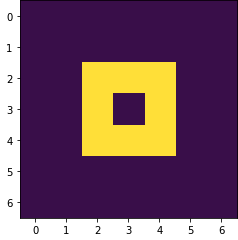
\includegraphics[width=\linewidth]{Materials/morphOrg}
		\caption{Original image.\newline}
	\end{subfigure}
	\hfill
	\begin{subfigure}{0.3\linewidth}
		\centering
		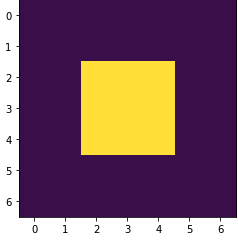
\includegraphics[width=\linewidth]{Materials/morphDilation}
		\caption{Original image after dilation and then erosion.}
	\end{subfigure}
	\hfill
	\begin{subfigure}{0.3\linewidth}
		\centering
		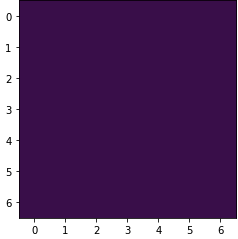
\includegraphics[width=\linewidth]{Materials/morphErosion}
		\caption{Original image after erosion and then dilation.}
	\end{subfigure}
	\caption{Example of applying dilation and then erosion is not the same as applying erosion and then dilation.}
	\label{dilationErosion}
\end{figure}
In a real scenario one might want to close holes in an initial segmentation of microvasculature (\autoref{microvasculature}) or in a brain (\autoref{brain}), but if one uses erosion on the microvasculature they risk disconnecting the vessels or even worse removing tips of the vessels. In the brain segmentation if dilation is used one risks the brain folds collapse and the brain becoming one big blob. Thus, care must be taken when segmenting thin objects not to make erosions, and care must be taken not to make dilations when details in a segmentation spatially lie very close to other details in the segmentation. However, when care \textit{is} taken, one can close the holes and remove leaks from their segmentation using dilation and erosion, and thus obtain an improved segmentation.

\begin{figure}[h]
	\centering
	\begin{subfigure}{0.3\linewidth}
		\centering
		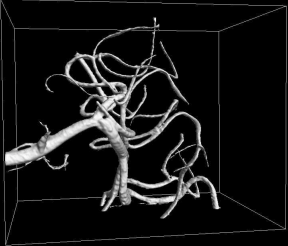
\includegraphics[width=\linewidth]{Materials/microvasculature}
		\caption{Initial segmentation of microvasculature.}
		\label{microvasculature}
	\end{subfigure}
	\hspace{1cm}
	\begin{subfigure}{0.3\linewidth}
		\centering
		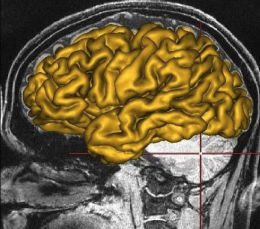
\includegraphics[width=\linewidth]{Materials/brain}
		\caption{Initial segmentation of a brain.}
		\label{brain}
	\end{subfigure}
	\caption{Examples of where care must be taken with dilation and erosion. Images taken from slides.}
\end{figure}
\section{Random walker}
Random walker is an algorithm which given seeds denoting different object classes has a 'walker' starting at a pixel location walking around the image with probabilities of where he is going proportional to the similarity between the pixel he is in and the neighbouring pixels. When he meets a seed, the class of the seed is recorded and after \textit{x} trials, the walker will begin in the next pixel of the image. Each pixel then gets the class its walkers reached most times out of the \textit{x} trials. This gives a segmentation of the whole image into any number of classes, but requires seeds are placed in the image beforehand. This describes an iterative solution for the algorithm, but a solution can be reached more efficiently solving the diffusion equation.\\
If we for instance want to segment the \textit{cell} image we need to first create an 'image' of seeds. This has been provided for us, but it only has one class (cell or not cell). We can thus use connected component decomposition to separate all connected points of seeds into their own class. We can then run the Random walker algorithm and we get a segmentation of each individual cell. This can be seen in \autoref{cellSeg}. As seen in the overlaid image we correctly find each of the cells we made seeds for, however, the quality of the segmentation is questionable as many cells are jagged, with some even having 90 degree angles. We also see quite a few leaks, and a few holes. However, the quality could be improved by using one or more erosions and then dilating the cells again, as this would remove the leaks and the rough edges and close the holes. We can also use Random walker for 3D segmentation, which can be seen in \autoref{mandible}, where we segment a mandible.

%\begin{figure}
%	\centering
%	\includegraphics[width=0.9\linewidth]{Materials/randomWalkerCell}
%	\caption{Seeds / markers used for random walker along with the original image, the final segmentation and all images overlaid.}
%	\label{cellSeg}
%\end{figure}
\begin{figure}
	\centering
	\begin{subfigure}{0.32\linewidth}
		\centering
		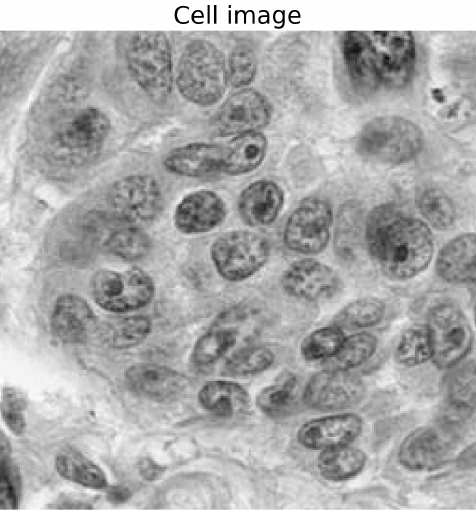
\includegraphics[width=\linewidth]{Materials/cell}
	\end{subfigure}
	\hfill
	\begin{subfigure}{0.32\linewidth}
		\centering
		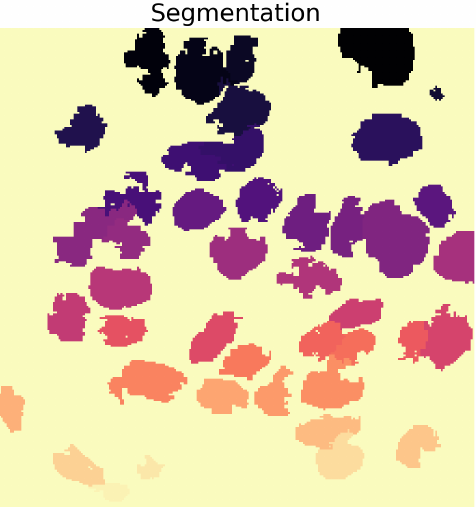
\includegraphics[width=\linewidth]{Materials/cellSeg}
	\end{subfigure}
	\hfill
	\begin{subfigure}{0.32\linewidth}
		\centering
		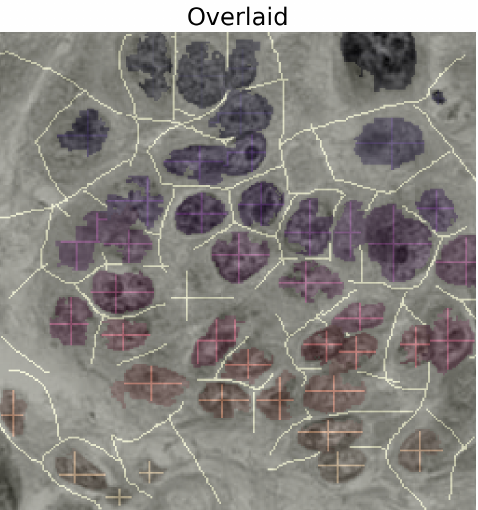
\includegraphics[width=\linewidth]{Materials/cellOverlaid}
	\end{subfigure}
	\caption{Original image, the final segmentation and markers, segmentation and original image overlaid.}
	\label{cellSeg}
\end{figure}

\begin{figure}
	\centering
	\begin{subfigure}{0.3\linewidth}
		\centering
		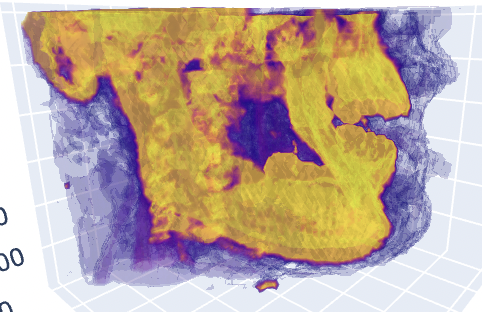
\includegraphics[width=\linewidth]{Materials/L3D}
		\caption{Right view on our data.}
	\end{subfigure}
	\hspace{1cm}
	\begin{subfigure}{0.3\linewidth}
		\centering
		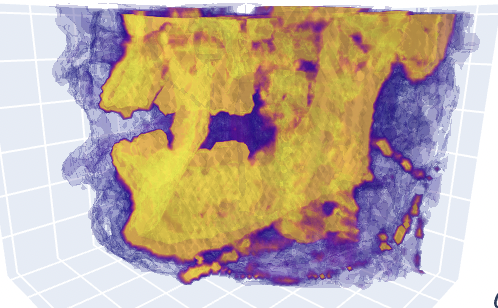
\includegraphics[width=\linewidth]{Materials/R3D}
		\caption{Left view on our data.\newline}
	\end{subfigure}
	\\
	\begin{subfigure}{0.3\linewidth}
		\centering
		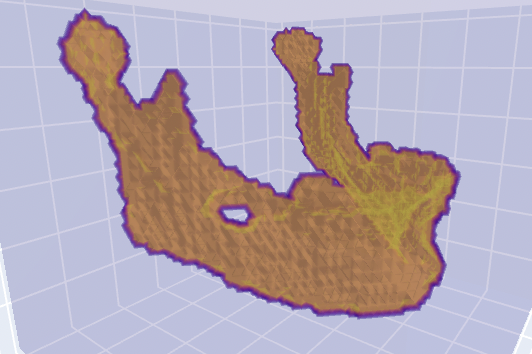
\includegraphics[width=\linewidth]{Materials/L3DSeg}
		\caption{Right view on segmentation.}
	\end{subfigure}
	\hfill
	\begin{subfigure}{0.3\linewidth}
		\centering
		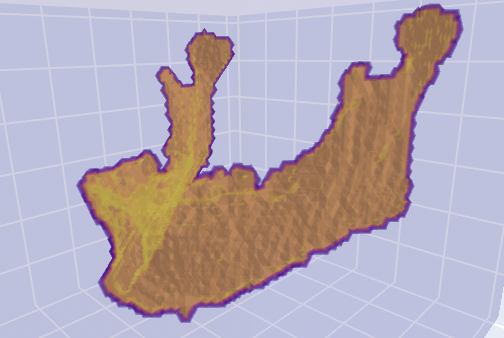
\includegraphics[width=\linewidth]{Materials/R3DSeg}
		\caption{Left view on Segmentation.}
	\end{subfigure}
	\hfill
	\begin{subfigure}{0.3\linewidth}
		\centering
		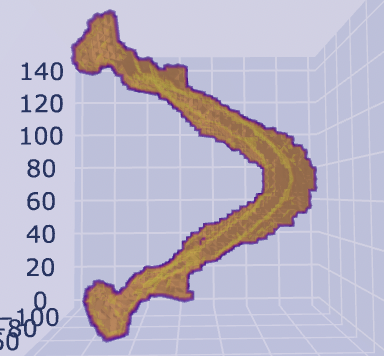
\includegraphics[width=\linewidth]{Materials/T3DSeg}
		\caption{Top view on segmentation.}
	\end{subfigure}
	\caption{Result of 3D segmentation of the mandible.}
	\label{mandible}
\end{figure}
Another algorithm which can be used for segmentation / to find object boundaries is Graph cut. Here the image is made to a graph representation and the more similar neighbouring pixels are, the more flow we allow between them. A max flow problem is then solved and a min cut is made to find the object boundary. As we are solving a max flow problem, this approach gives us an analytical solution to our segmentation problem opposed to the non-deterministic approach of using Random walker. This is a big advantage as the solution to the problem becomes consistent, however, it also requires it is possible to make a graph representation of the image and that it is possible to come up with a cost function. And even if this is possible, it requires that the graph representation can be contained in memory to be solved efficiently. Another issue could be boundaries are not 'clear' and a high amount of flow would go through what is supposed to be our boundaries, making it hard to make a min cut at an exact location. These issues are not present in the Random walker.\\
In conclusion, the Graph cut algorithm is preferred as it gives us an analytical solution, however it is not always possible to employ the Graph cut algorithm due to memory usage, cost function formulation or vague boundaries, but the Random walker algorithm solves these issues by being non-deterministic.
\section{PCA}
PCA is a procedure which captures the directions of greatest data variability. That is, having a high dimensional dataset and performing an PCA would give us the eigenvectors and eigenvalues explaining the variance in the data. We can then choose to keep the eigenvectors that explain, say, 98\% of the variance in the data, and because the first few components / eigenvectors explain the vast majority of the variance, this will often lead to a big dimensionality reduction of the data.\\
In medical image analysis we can obtain such a high dimensionality dataset if we describe a shape by several data points / landmarks. If we were to describe a lung field, this could be done with 100 points in 2D giving us a 200 dimensional dataset for each lung field we describe. If we have several lung fields described in this manner, we can now normalize them using a Procrustes analysis and then perform PCA. In the data we are given, we have 124 lung fields described by 94 points. After performing PCA and retaining 98\% of the variance we find 20 components are enough. We can now visualize how adjusting the magnitude of the principal components affects our lungs. In \autoref{PCA} we see how the first three principal components affects our lung shape. These are the components which describes most of our variance in the data, and thus the components which gives the biggest change in shape.

\begin{figure}[h]
	\centering
	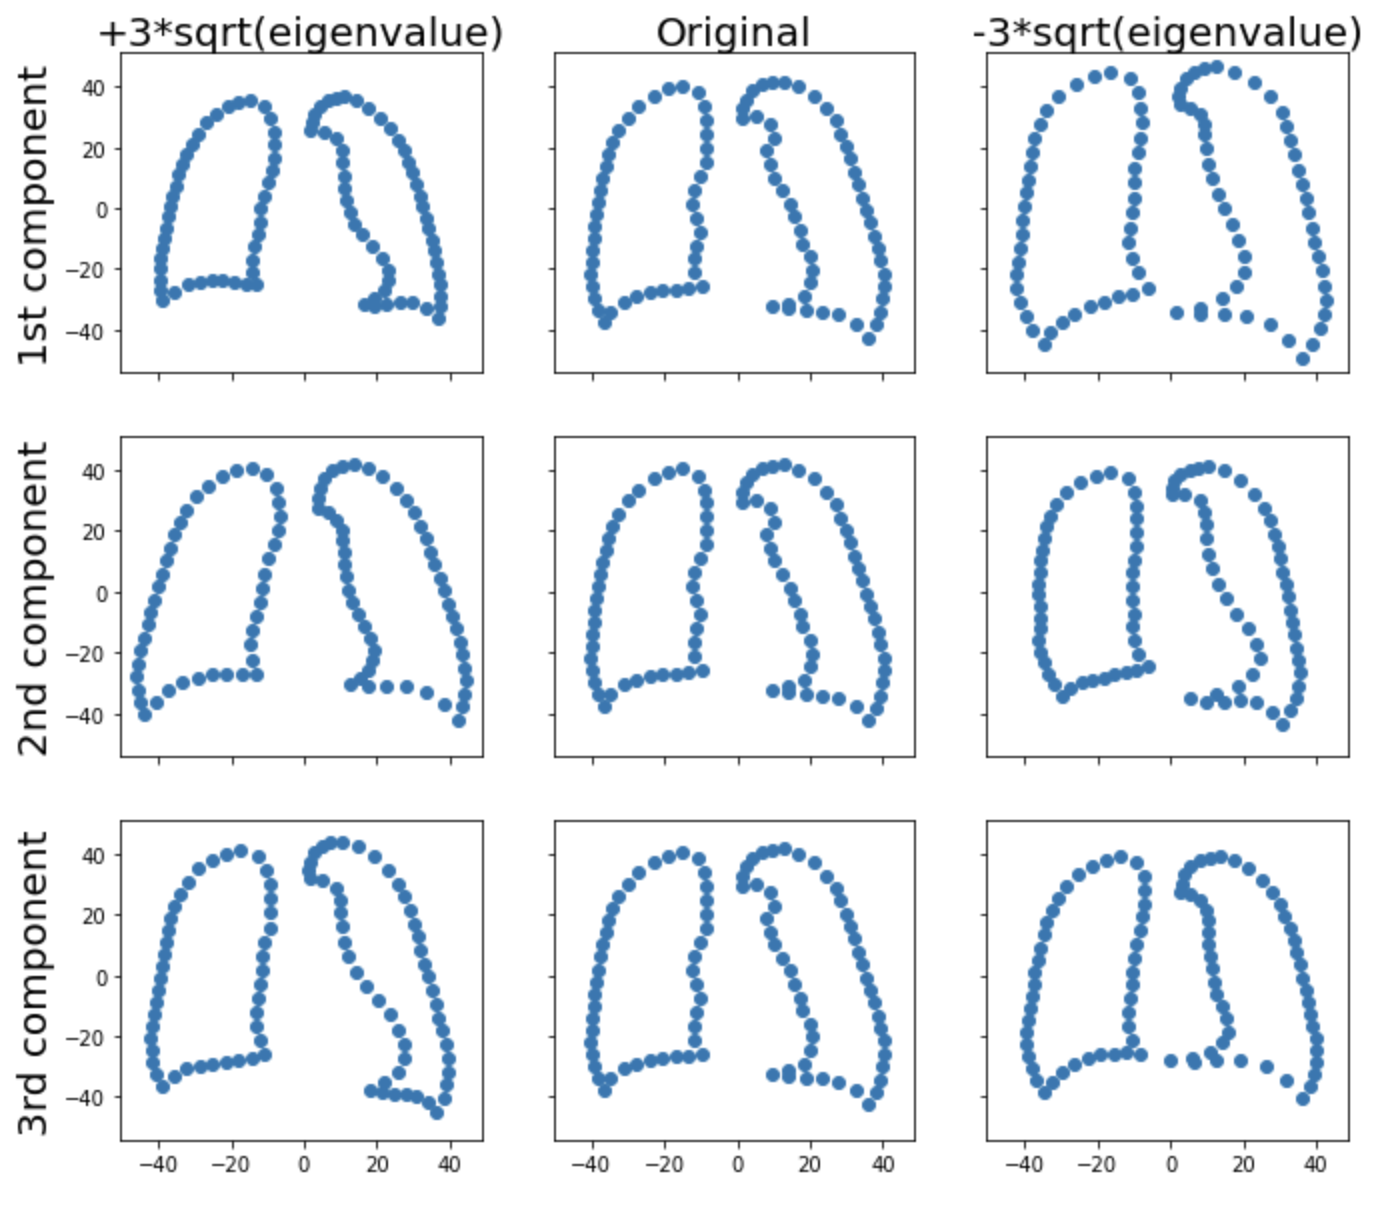
\includegraphics[width=0.73\linewidth]{Materials/PCA}
	\caption{How the first three principal components affects the shape of our lung.}
	\label{PCA}
\end{figure}
Using the 20 components describing 98\% of the variance in our lung fields we can now fit a mean lung shape, the lung found by taking the average shape of our lungs, to a never-before-seen lung and because we fit it using the components we avoid fitting to noise. We can then make an error measure of how well this active shape model / our mean lung fits our new lung, and use this to determine if we are seeing a healthy or sick lung / a normal or abnormal lung. Fitting our active shape model also gives a good boundary segmentation of the new lung. Even just using the mean lung shape would give a decent initial segmentation of a new lung field in most cases.
\section{Conclusion}
In conclusion we have seen where segmentation can be used in medical image analysis, we have seen the risks of dilation and erosion and explained the benefits of them, we have concluded Graph cut segmentations are preferred, but also have limited applications and Random walker alleviates these constrains by being non-deterministic, and finally we have looked into how PCA can be used for segmentation.
\newpage
\section{Code collaboration}
The code for this assignment has been developed in collaboration with: Marcus Hansen, Ulrik Larsen and Sarah Hansen
%
% ---- Bibliography ----
%
% BibTeX users should specify bibliography style 'splncs04'.
% References will then be sorted and formatted in the correct style.
%
% \bibliographystyle{splncs04}
% \bibliography{mybibliography}
%
\begin{thebibliography}{8}
\bibitem{MIA}
A.P. Dhawan, Medical Image Analysis, 2nd edition, 2011, John Wiley

\bibitem{MIS}
A. Maier, et al., Medical Imaging Systems, 2018, Springer Open

\bibitem{otherExamples}
A. Norouzi, et. al., 'Medical Image Segmentation Methods, Algorithms, and Applications', IETE Technical Review, Volume 31, Issue 3, 23 June 2014.

\end{thebibliography}
\end{document}
